% \section{Цель работы}
% \begin{frame}[plain]
%     \frametitle{Цель работы}
%         Исследование и совершенствование методов оптимизации для задач большой размерностью, не обладающих достаточной гладкостью для применения классических методов. Предприняты шаги по расширению доступного класса задач, рассматриваются аналоги условия Липшица, которые позволяют сохранить свойственную липшицевым задачам оптимальные оценки скорости сходимости.
% \end{frame}

\begin{frame}{[1 глава] Введение и Обзор Литературы.}
    Описывается философия, стоящая за оракульной сложностью. 
    
    В силу роста популярности задач большой размерности, большей значимостью является развитие методов первого порядка.
    Поэтому обозревается постановка и устройство таких методов, как:
    \begin{itemize}
        \item градиентный спуск
        \item наискорейший спуск
        \item ускоренные и моментные методы
        \item метод Ньютона
        \item квазиньютоновские методы(BFGS)
    \end{itemize}
\end{frame}


\begin{frame}{[1 глава] Минимизация силового поля.}
    \begin{figure}
    \begin{center}
        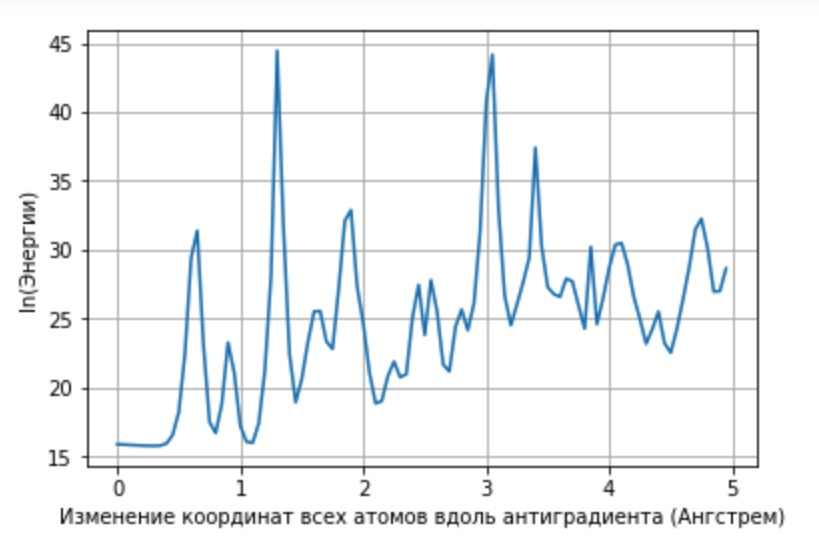
\includegraphics[width=0.85\linewidth]{1DSearch.jpg}
    \end{center}
    \end{figure}
    \begin{table}[h]
    \centering
    \resizebox{\textwidth}{!}{
        \begin{tabular}{|c|c|c|}
            \hline
            \fontsize{12pt}{12pt}\selectfont {\bfseries Показатели} & {\bfseries ``Шевеление'' атома} & {\bfseries Адаптивный градиентный спуск} \\
            \hline
            \fontsize{12pt}{12pt}\selectfont Время 1 итерации, секунды    & 1.2075 & 122.9814 \\
            \hline
            \fontsize{12pt}{12pt}\selectfont Энергия 1 итерации, кДж/моль & 0.0225 & 2.7081 \\
            \hline
            \fontsize{12pt}{12pt}\selectfont $\sim\Delta$Энергии к 300 минуте, кДж/моль & $- 347$ & $- 413$ \\
            \hline
        \end{tabular}
    }
    \end{table}
\end{frame}


\begin{frame}{[2 глава] Оптимальная оценка.}
    В работе \href{https://arxiv.org/abs/1212.2002}{[Lacoste-Julien et al., 2012]} был предложен \textbf{оптимальный} субградиентый метод для:
    \begin{itemize}
        \item задач \textbf{сильно выпуклой} минимизации
        \item в предположении \textbf{липшицевости} целевого функционала
    \end{itemize}
    Задача: $$\min_{x \in Q} f(x)$$
    Метод: $$ x_{k+1} = {Proj}_{Q}(x_k - h_k \nabla f(x_k) ), \; \; где h_k = \frac{2}{\mu (k+1)} $$
\end{frame}


\begin{frame}{[2 глава] Оптимальная оценка.}
    Оценка скорости сходимости: 
    $$
    \label{eq:1} f(\widehat{x}) - f(x_*) \leq \frac{2 M^2}{\mu (N+1)} \; \forall x \in Q,
    $$
    
    где $$\widehat{x} = \sum_{k=1}^{N} \frac{2 k}{N (N+1)} \; x_k,  \;\;\;\;\;\; \norm{\nabla f(x)}_{2} \leq M \; \forall x \in Q,$$
    $N$ --- количество итераций, \\
    $\mu$ --- константа сильной выпуклости $f(x)$ 
\end{frame}


\begin{frame}{[2 глава] Обобщение.}
    Верхняя оценка скорости сходимости: 
    $$
    f(\widehat{x}) - f(x_*) \leq \frac{2 M^2}{\mu (N+1)} \; \forall x \in Q,
    $$
    Зеркальный спуск в общем случае:
    $$
    x_{k+1} := \argmin_{x \in Q} \{ h_k \langle \nabla f(x_k), x\rangle + V(x, x_k)\} 
    $$
    где $V(y,x) = d(y) - d(x) - \langle \nabla d(x), y - x \rangle$ --- дивергенция Брэгмана, причем $d()$ --- выпуклая прокс-функция.
\end{frame}


\begin{frame}{[2 глава] Необходимые определения.}
    \begin{block}{[Определение] Относительная Липшицевость  \href{https://arxiv.org/pdf/1710.04718.pdf}{[Lu, 2018]}}
        $$
        \langle \nabla f(x), x - y \rangle \leq M\sqrt{2 V(y, x)} \;\;\; \forall x, y \in Q
        $$
    \end{block}

    \begin{exampleblock}{Пример. Функция относительно липшицева, но не липшицева.} 
        Пусть $f(x) := x^2$ для $x \in \mathbb{R}$. Производная $f$ неограничена на $\mathbb{R}$, она не является липшицевой на всей прямой. Введем $d$ как $d(x) := 2x^4$
        Тогда
        $$ V(y, x) = 2y^4 - 2x^4 - 8x^3 (y-x) = \frac{1}{2}(x^2 - y^2) + x^2 (x - y)^2 \geq x^2 (x - y)^2 $$
        Значит, $ (f'(x) (x - y))^2 = 4x^2 (x - y)^2 \leq 2 \cdot 2 V(y,x)$ \\
        \vspace{\baselineskip}
        \centering{ Следовательно $f$ --- $\sqrt{2}$-относительно липшицева.}
    \end{exampleblock}
\end{frame}


\begin{frame}{[2 глава] Необходимые определения.}
    \begin{block}{[Определение] Относительная сильная выпуклость \href{https://arxiv.org/pdf/1610.05708.pdf}{[Lu et al., 2018]}}
        $$
         f(y) \geq f(x) + \langle \nabla f(x), y - x \rangle + \mu V(y, x) \;\;\; \forall x, y \in Q
        $$
    \end{block}
    \begin{exampleblock}{Пример. Функция относительно липшицева и относительно сильно выпукла. \href{https://proceedings.neurips.cc/paper/2020/file/b67fb3360ae5597d85a005153451dd4e-Paper.pdf}{[Zhou et al., 2020]}} 
        Пусть $f(x) := \frac{1}{p}\norm{\cdot}^p_2$ для $p \geq 2$ и $ Q = [-\alpha, \alpha], \; \alpha \ge 0$. Заметим, что $\nabla f(x) = \norm{x}_2^{p - 2} x$ и $\nabla^2 f(x) = \norm{x}_2^{p - 2} I + (p-2)\norm{x}_2^{p - 4} x x^{T}$\\
        $f$ --- является относительно липшицевой с $M = 1$ и $d := \frac{1}{2p}\norm{\cdot}_2^{2p}$\\
        $f$ --- не является сильно выпуклой, т.к. $\nabla^2 f(x) - \mu I$ не является положительно полуопределенной в окрестности 0, но можно подобрать $\mu$, которое удовлетворяет данному условию.
    \end{exampleblock}
\end{frame}


\begin{frame}{[2 глава] Необходимые определения.}
    \begin{block}{[Определение] Относительная сильная монотонность}
        $$ \mu V(y, x) + \mu V(x, y) \leq \langle g(y) - g(x), y - x \rangle  \forall x, y \in Q,$$
    \end{block}
    \begin{exampleblock}{Пример}
        Рассмотрим $f$ --- $\mu$-относительно сильно выпуклая \\$f(x) - f(y) + \mu V(x, y) \leq \langle \nabla{f(x)}, x - y \rangle  \;\; \forall x, y \in Q, $
        то
        $$f(y) - f(x) + \mu V(y, x) \leq \langle \nabla{f(y)}, y - x \rangle  \forall x, y \in Q, $$
        После сложения последних неравенств, получаем
        $$\mu V(x, y) + \mu V(y, x)\leq \langle \nabla{f(y)} - \nabla{f(x)}, y - x \rangle \;\; \forall x, y \in Q,$$
    \end{exampleblock}
\end{frame}


\begin{frame}{[2 глава] Мотивация для работы с ВН.}
    \begin{exampleblock}{Пример. Функция Лагранжа}
        Функционалы относительно сильно выпуклы:
        $$
        \left\{\begin{aligned}
            \min_{x \in Q} \widehat{g}(x)\\
             g_1(x){,\:}g_2(x){,\:}...\:g_m(x) \leq 0
        \end{aligned}\right.
        $$
        $$L(x, \lambda) = \min_{x \in Q} \max_{\overrightarrow{\lambda} \in \mathbb{R}_+^n} \widehat{g}(x) + \sum_{p=1}^{m} \lambda_p g_p(x) + \varepsilon \norm{V(x)}_*^2$$
    \end{exampleblock}
    Введем оператор:
    $ g(x) := \Bigg( 
      \begin{aligned}
        f^{'}_{u}(u,v)&&\\
        -f^{'}_{v}(u,v)&&
      \end{aligned}
      \Bigg) $
    и ВН: $\langle g(x), x - y \rangle \leq 0$
\end{frame}


\begin{frame}{[2 глава] Теорема для обобщенного случая.}
    \begin{block}{[Теорема]}
        Пусть $g$ --- $\mu$-относительно сильно монотонный оператор и $M$-относительно ограниченный. Тогда после $N$ итераций алгоритма: 
        $$ x_{k+1} := \argmin_{x \in Q} \{ h_k \langle g(x_k), x\rangle + V(x, x_k)\}, \;\;\; h_k = \frac{2}{\mu (k+1)}$$
        будет верно неравенство:
        \begin{equation}\label{eq:2}
            \max_{x \in Q} \langle g(x), \widehat{x} - x\rangle \leq \frac{2 M^2}{\mu (N+1)}
        \end{equation}
    \end{block}
\end{frame}


\begin{frame}{[2 глава] Уточнение оценки при доп. условиях.}
    \begin{block}{[Следствие]}
         $ \max_{x \in Q} \langle g(x), \widehat{x} - x\rangle \leq \varepsilon$
        после $N = \mathcal{O}(\frac{M^2}{\mu \varepsilon})$
    \end{block}
    \begin{block}{[Замечание]}
        Если $d$ --- 1-сильно выпукла и $\norm{g(x)}_* \leq M$, то оценку \eqref{eq:2} можно уточнить
        \begin{equation}
            \max_{x \in Q} \langle g(x), \widehat{x} - x\rangle \leq \frac{2}{\mu N (N+1)} \sum_{k=1}^{N} \frac{k}{k+1} \norm{g(x_k)}_*^2
        \end{equation}
    \end{block}
\end{frame}


\begin{frame}{[2 глава] Уточненная оценка.}
    Уточненная (адаптивная) верхняя оценка скорости сходимости: 
    $$
    f(\widehat{x}) - f(x_*) \leq \frac{2}{\mu N (N+1)} \sum_{k=1}^{N} \frac{k \norm{\nabla f(x_k)}_*^2 }{k+1}\;\;\; \forall x \in Q,
    $$
\end{frame}


\begin{frame}{[2 глава] Эксперименты. Удаленность от решения.}
\begin{figure}
    \centering
    \includegraphics[width=1\linewidth]{"compare_radius"}
\end{figure}
\end{frame}


\begin{frame}{[2 глава] Эксперименты. Неограниченное Q.}
\begin{columns}
    \begin{column}{0.55\textwidth}
    \begin{figure}
        \centering
        \includegraphics[width=1\linewidth]{"q_unlim"}
    \end{figure}
    \end{column}
        
    \begin{column}{0.55\textwidth}
    \begin{figure}
        \centering
        \includegraphics[width=1\linewidth]{"q_unlim_raw"}
    \end{figure}
    \end{column}
\end{columns}
\end{frame}


\begin{frame}{[3 глава] Дальнейшее направление работы.}
    \begin{block}{[Определение] Условие острого минимума \href{https://doi.org/10.1016/0041-5553(69)90061-5}{[Polyak, 1969]}}
        \begin{equation}
            f(x) - f(x_*) \geq \alpha \min_{x_* \in X_*}{\| x - x_* \|_2} \text{ при } \alpha > 0\;\; \forall x \in Q
        \end{equation}
    \end{block}
    \begin{block}{[Определение] Условие $\gamma$-роста}
       \begin{equation} \label{gamma-growth}
           f(x) - f(x_*) \geq \mu_{\gamma}\left(\min_{x_* \in X_*}{V(x_*,x)}\right)^{\gamma/2} \text{ при } \gamma \geq 1\;\; \forall x \in Q
       \end{equation}
    \end{block}
\end{frame}

\begin{frame} {[3 глава] Сильная выпуклость и острый минимум.}
    \begin{figure}[H]
        \minipage{0.49\textwidth}
        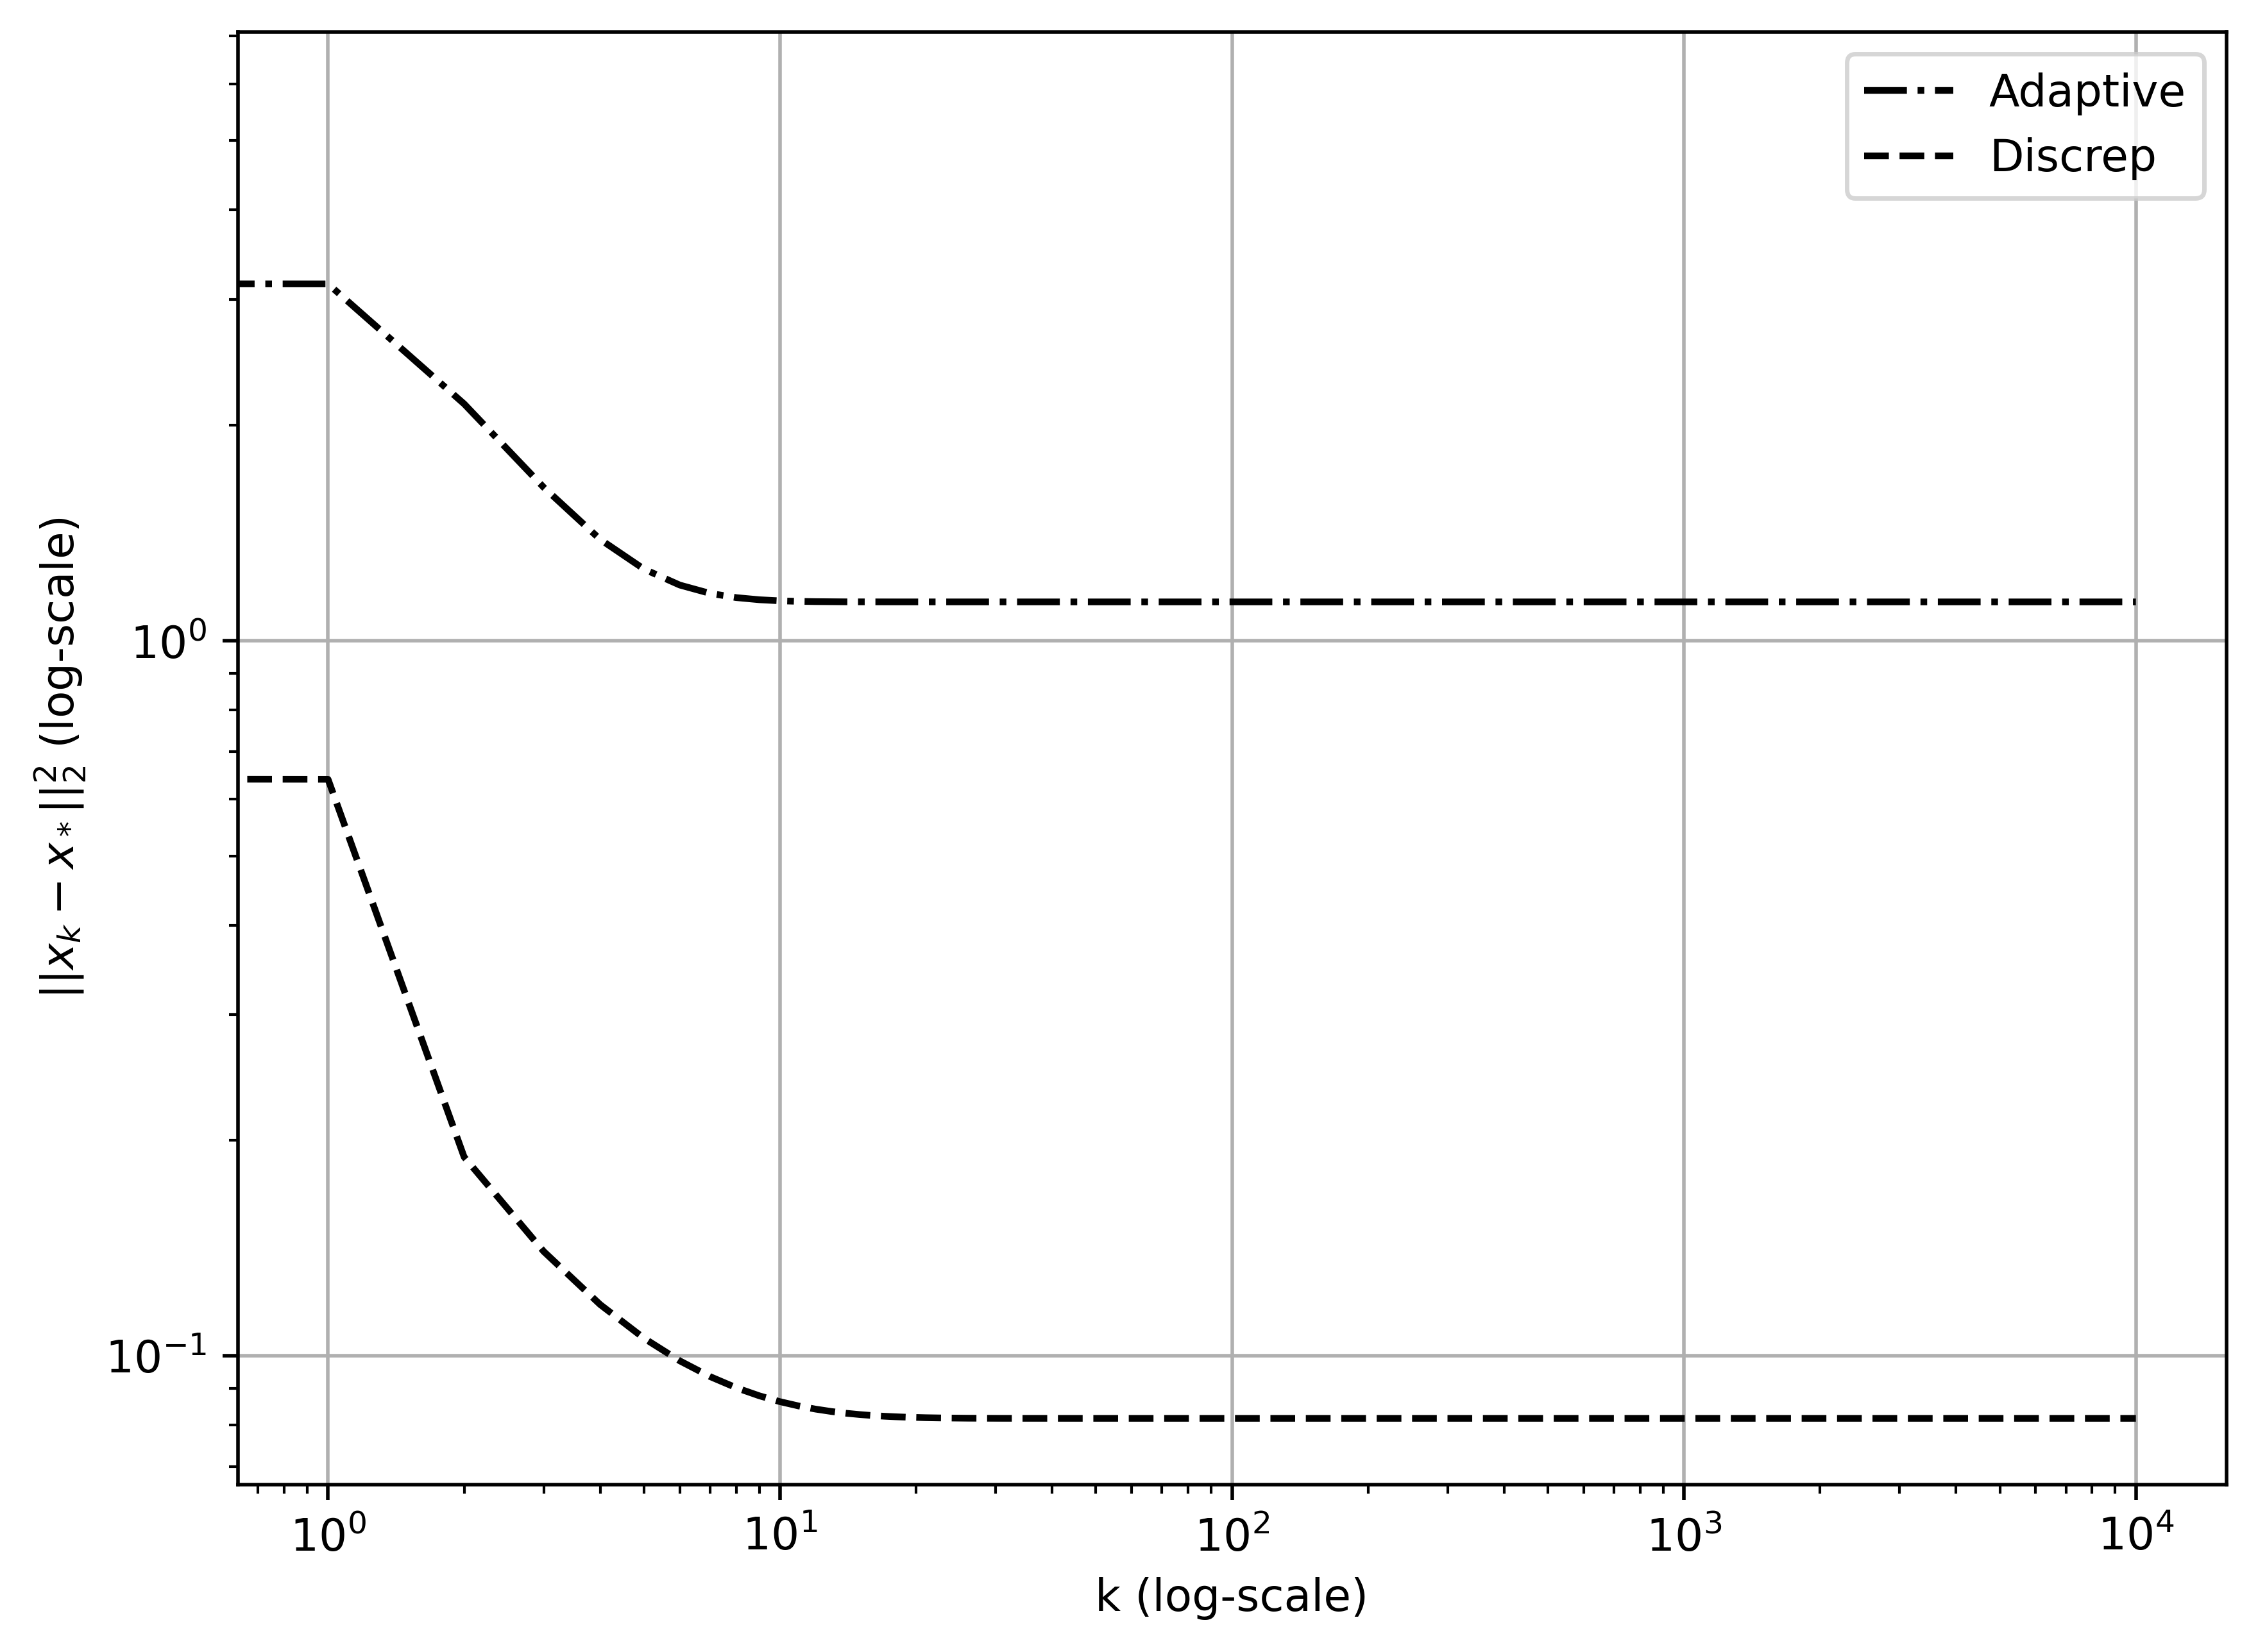
\includegraphics[width=\linewidth]{sharp_convex_x.png}
        \endminipage\hfill
        \minipage{0.49\textwidth}
        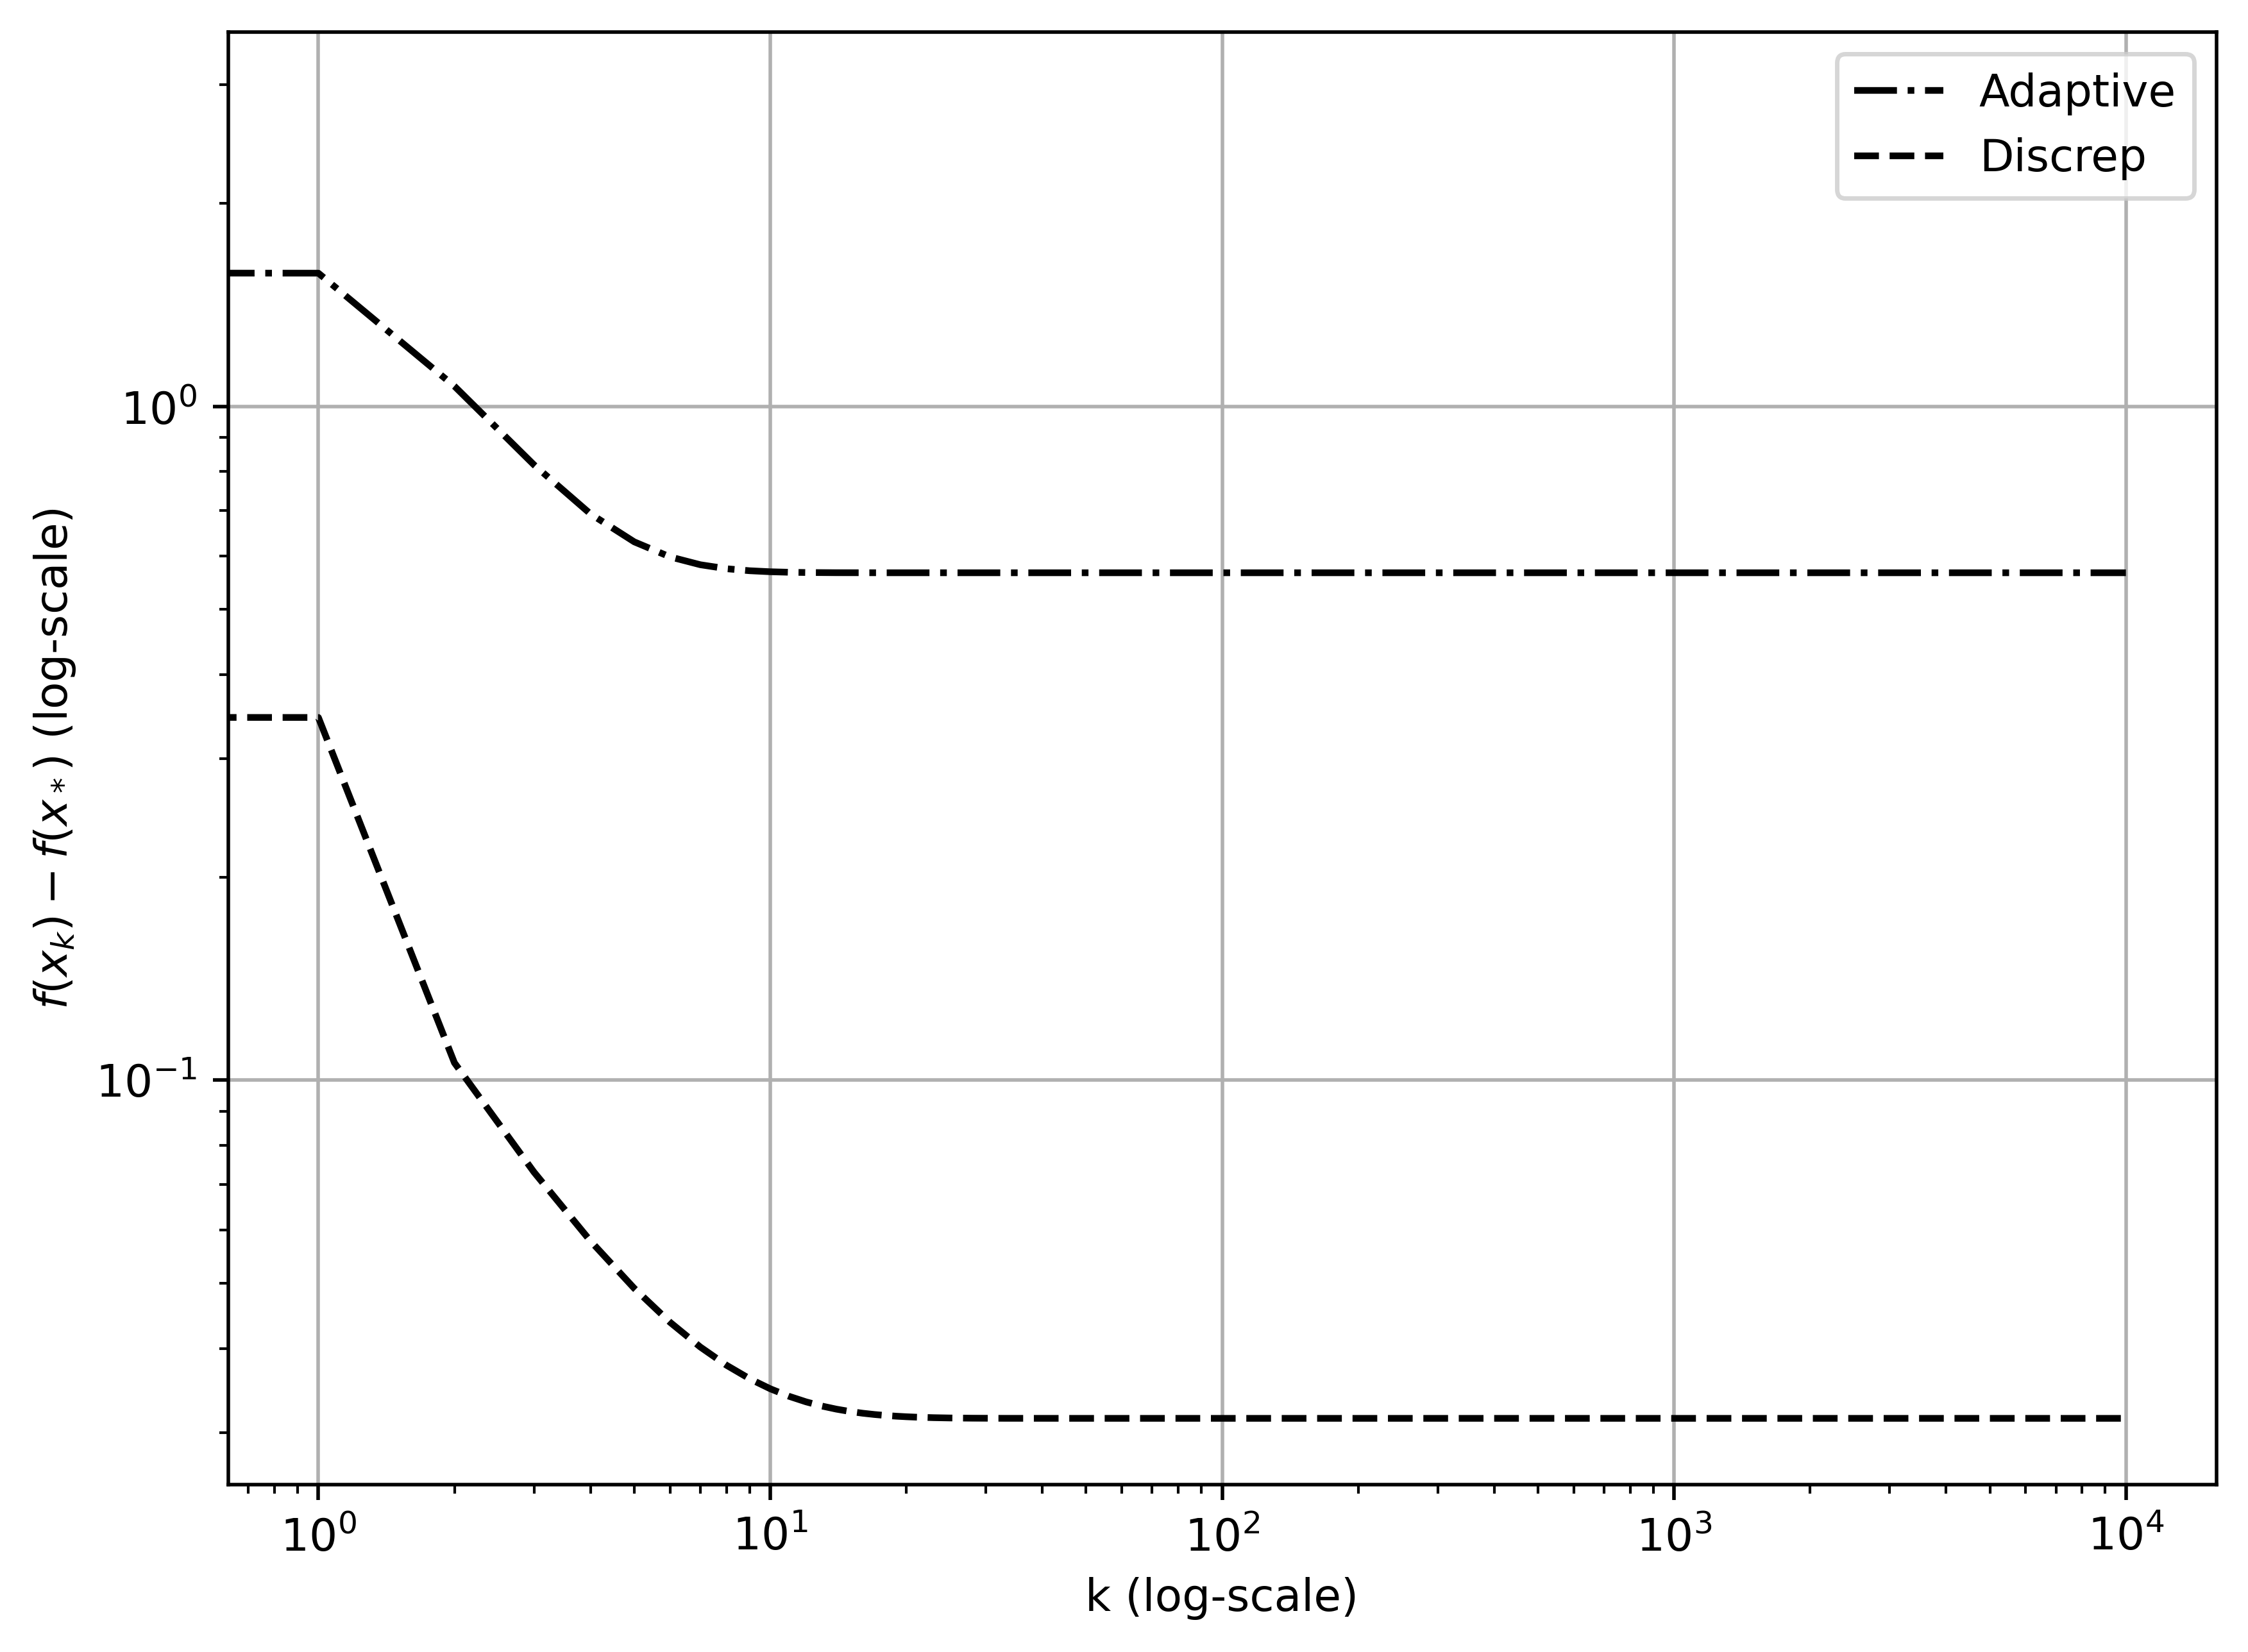
\includegraphics[width=\linewidth]{sharp_convex_f.png}
        \endminipage\hfill
        \label{res_sharp_convex}
    \end{figure}
    
    \begin{figure}[H]
        \minipage{0.49\textwidth}
        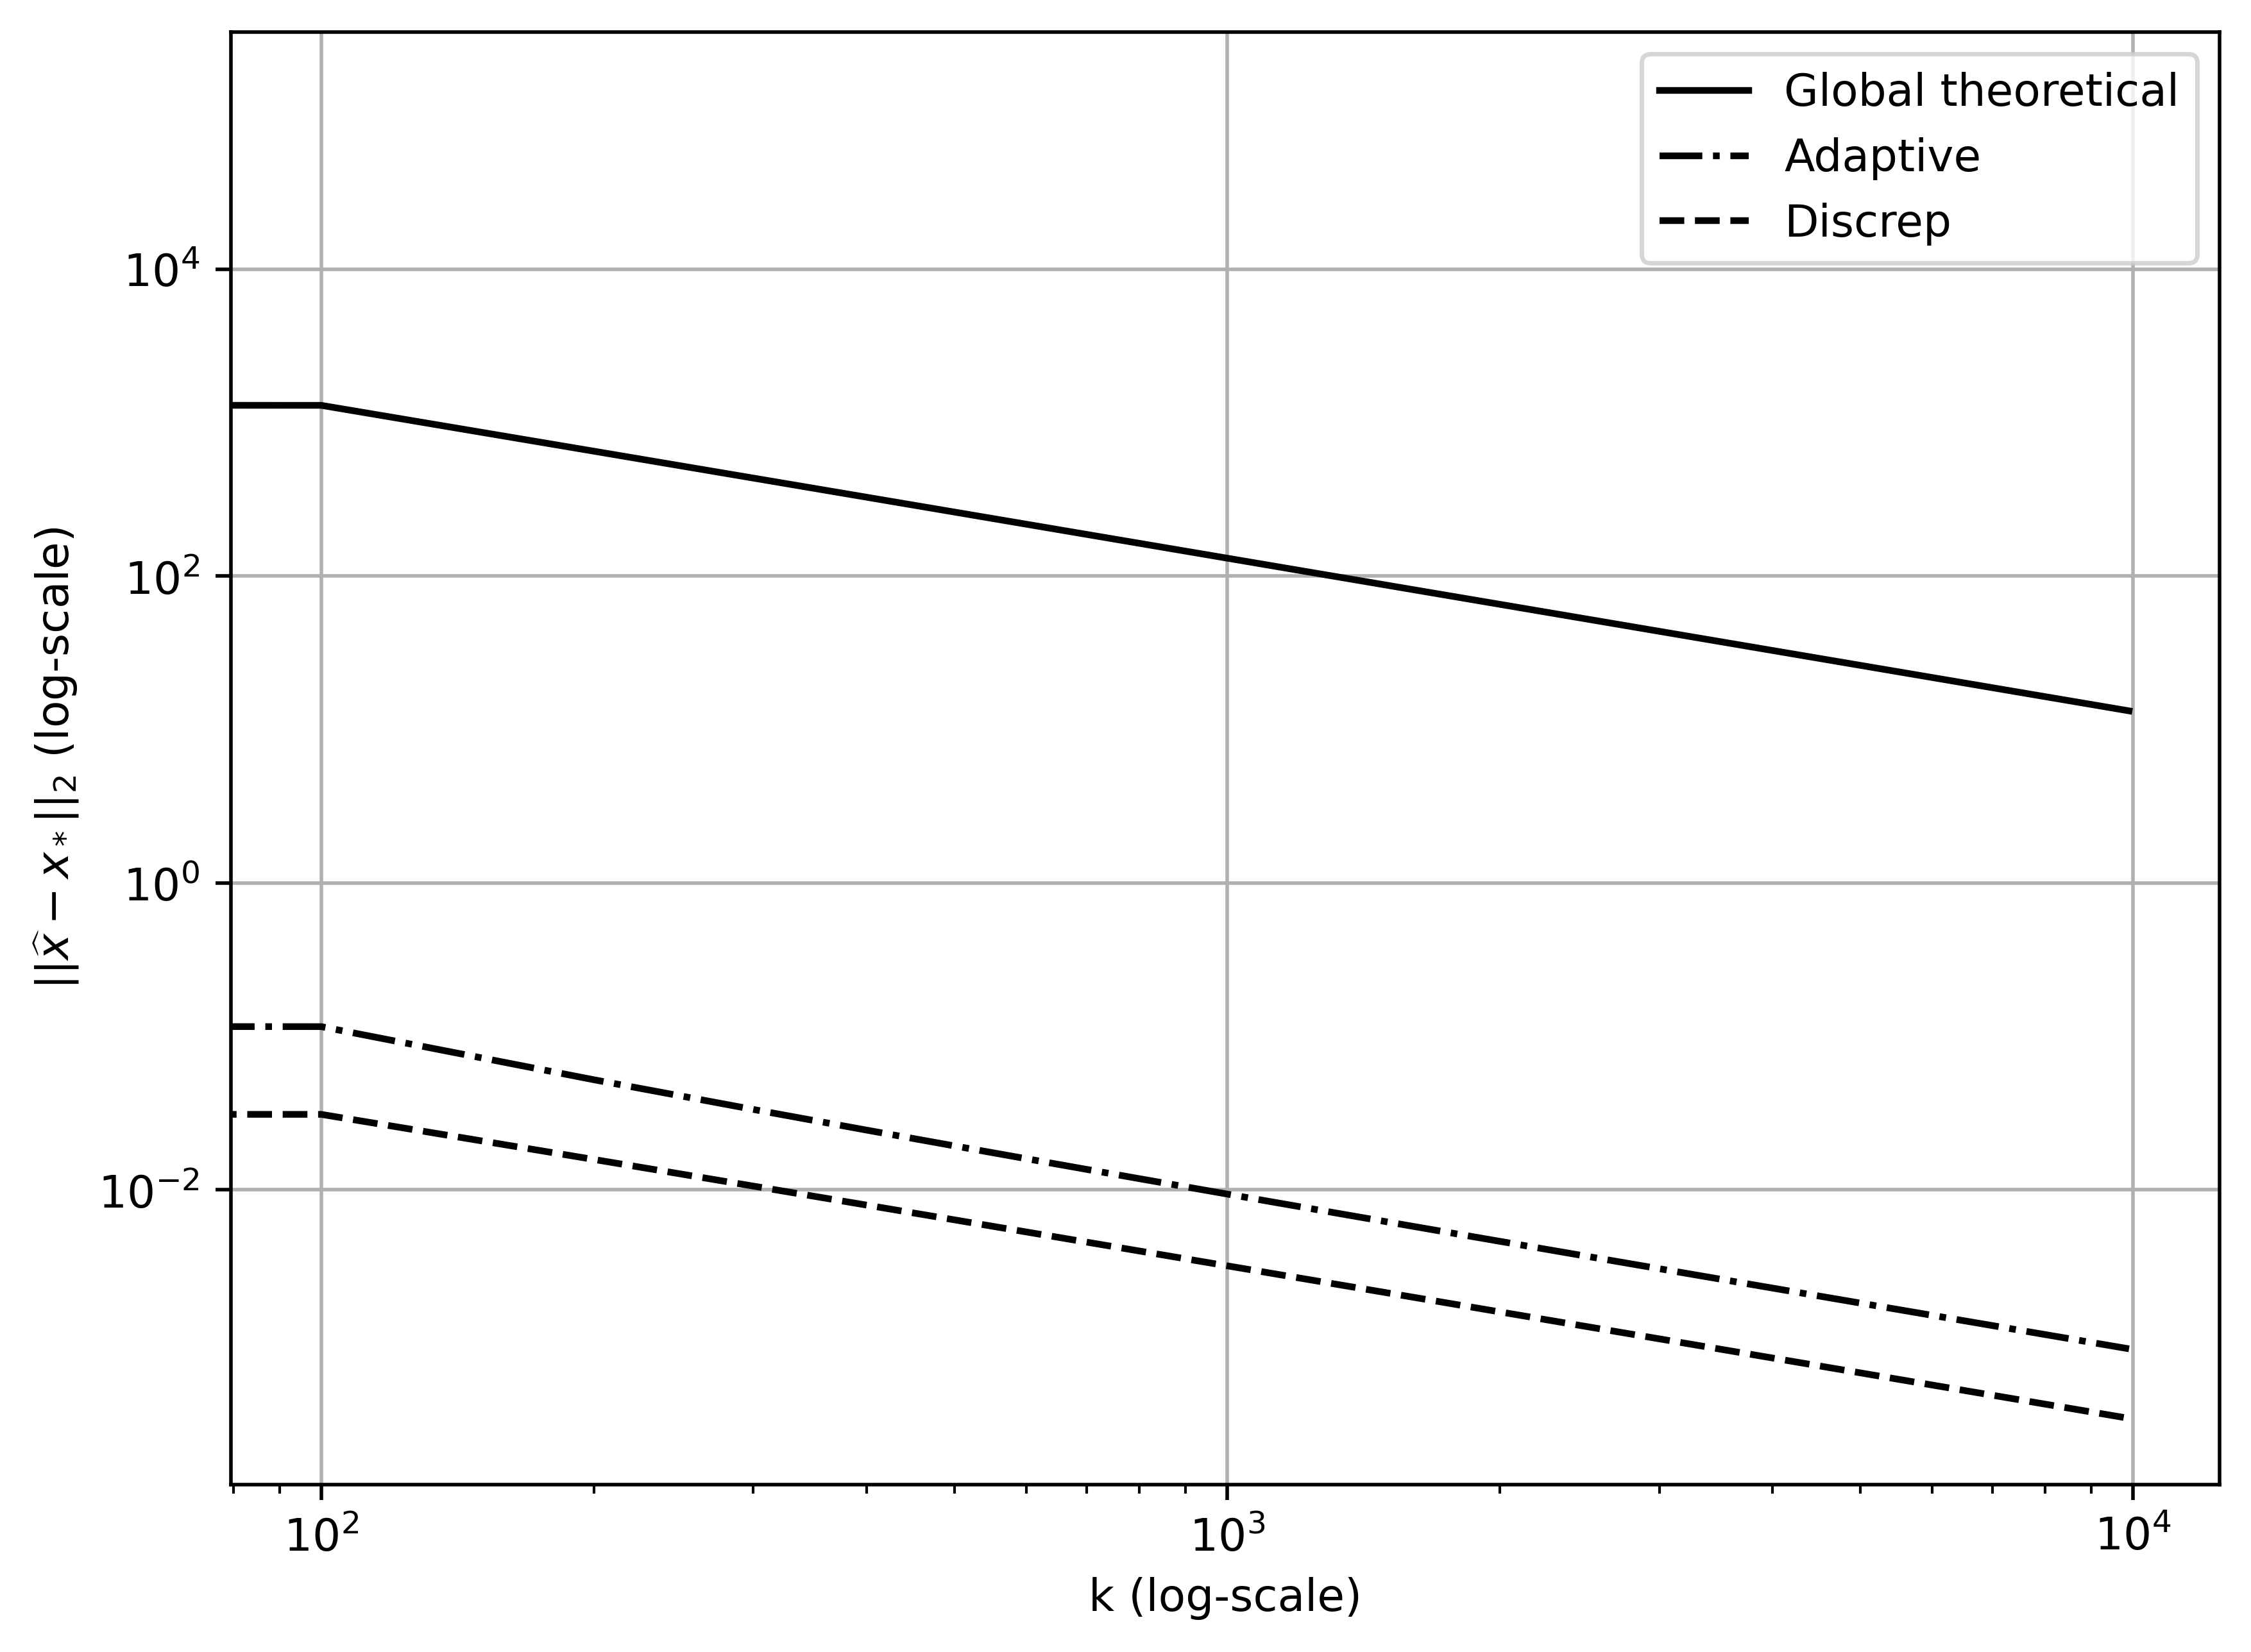
\includegraphics[width=\linewidth]{strong_convex_small_rad_x.png}
        \endminipage\hfill
        \minipage{0.49\textwidth}
        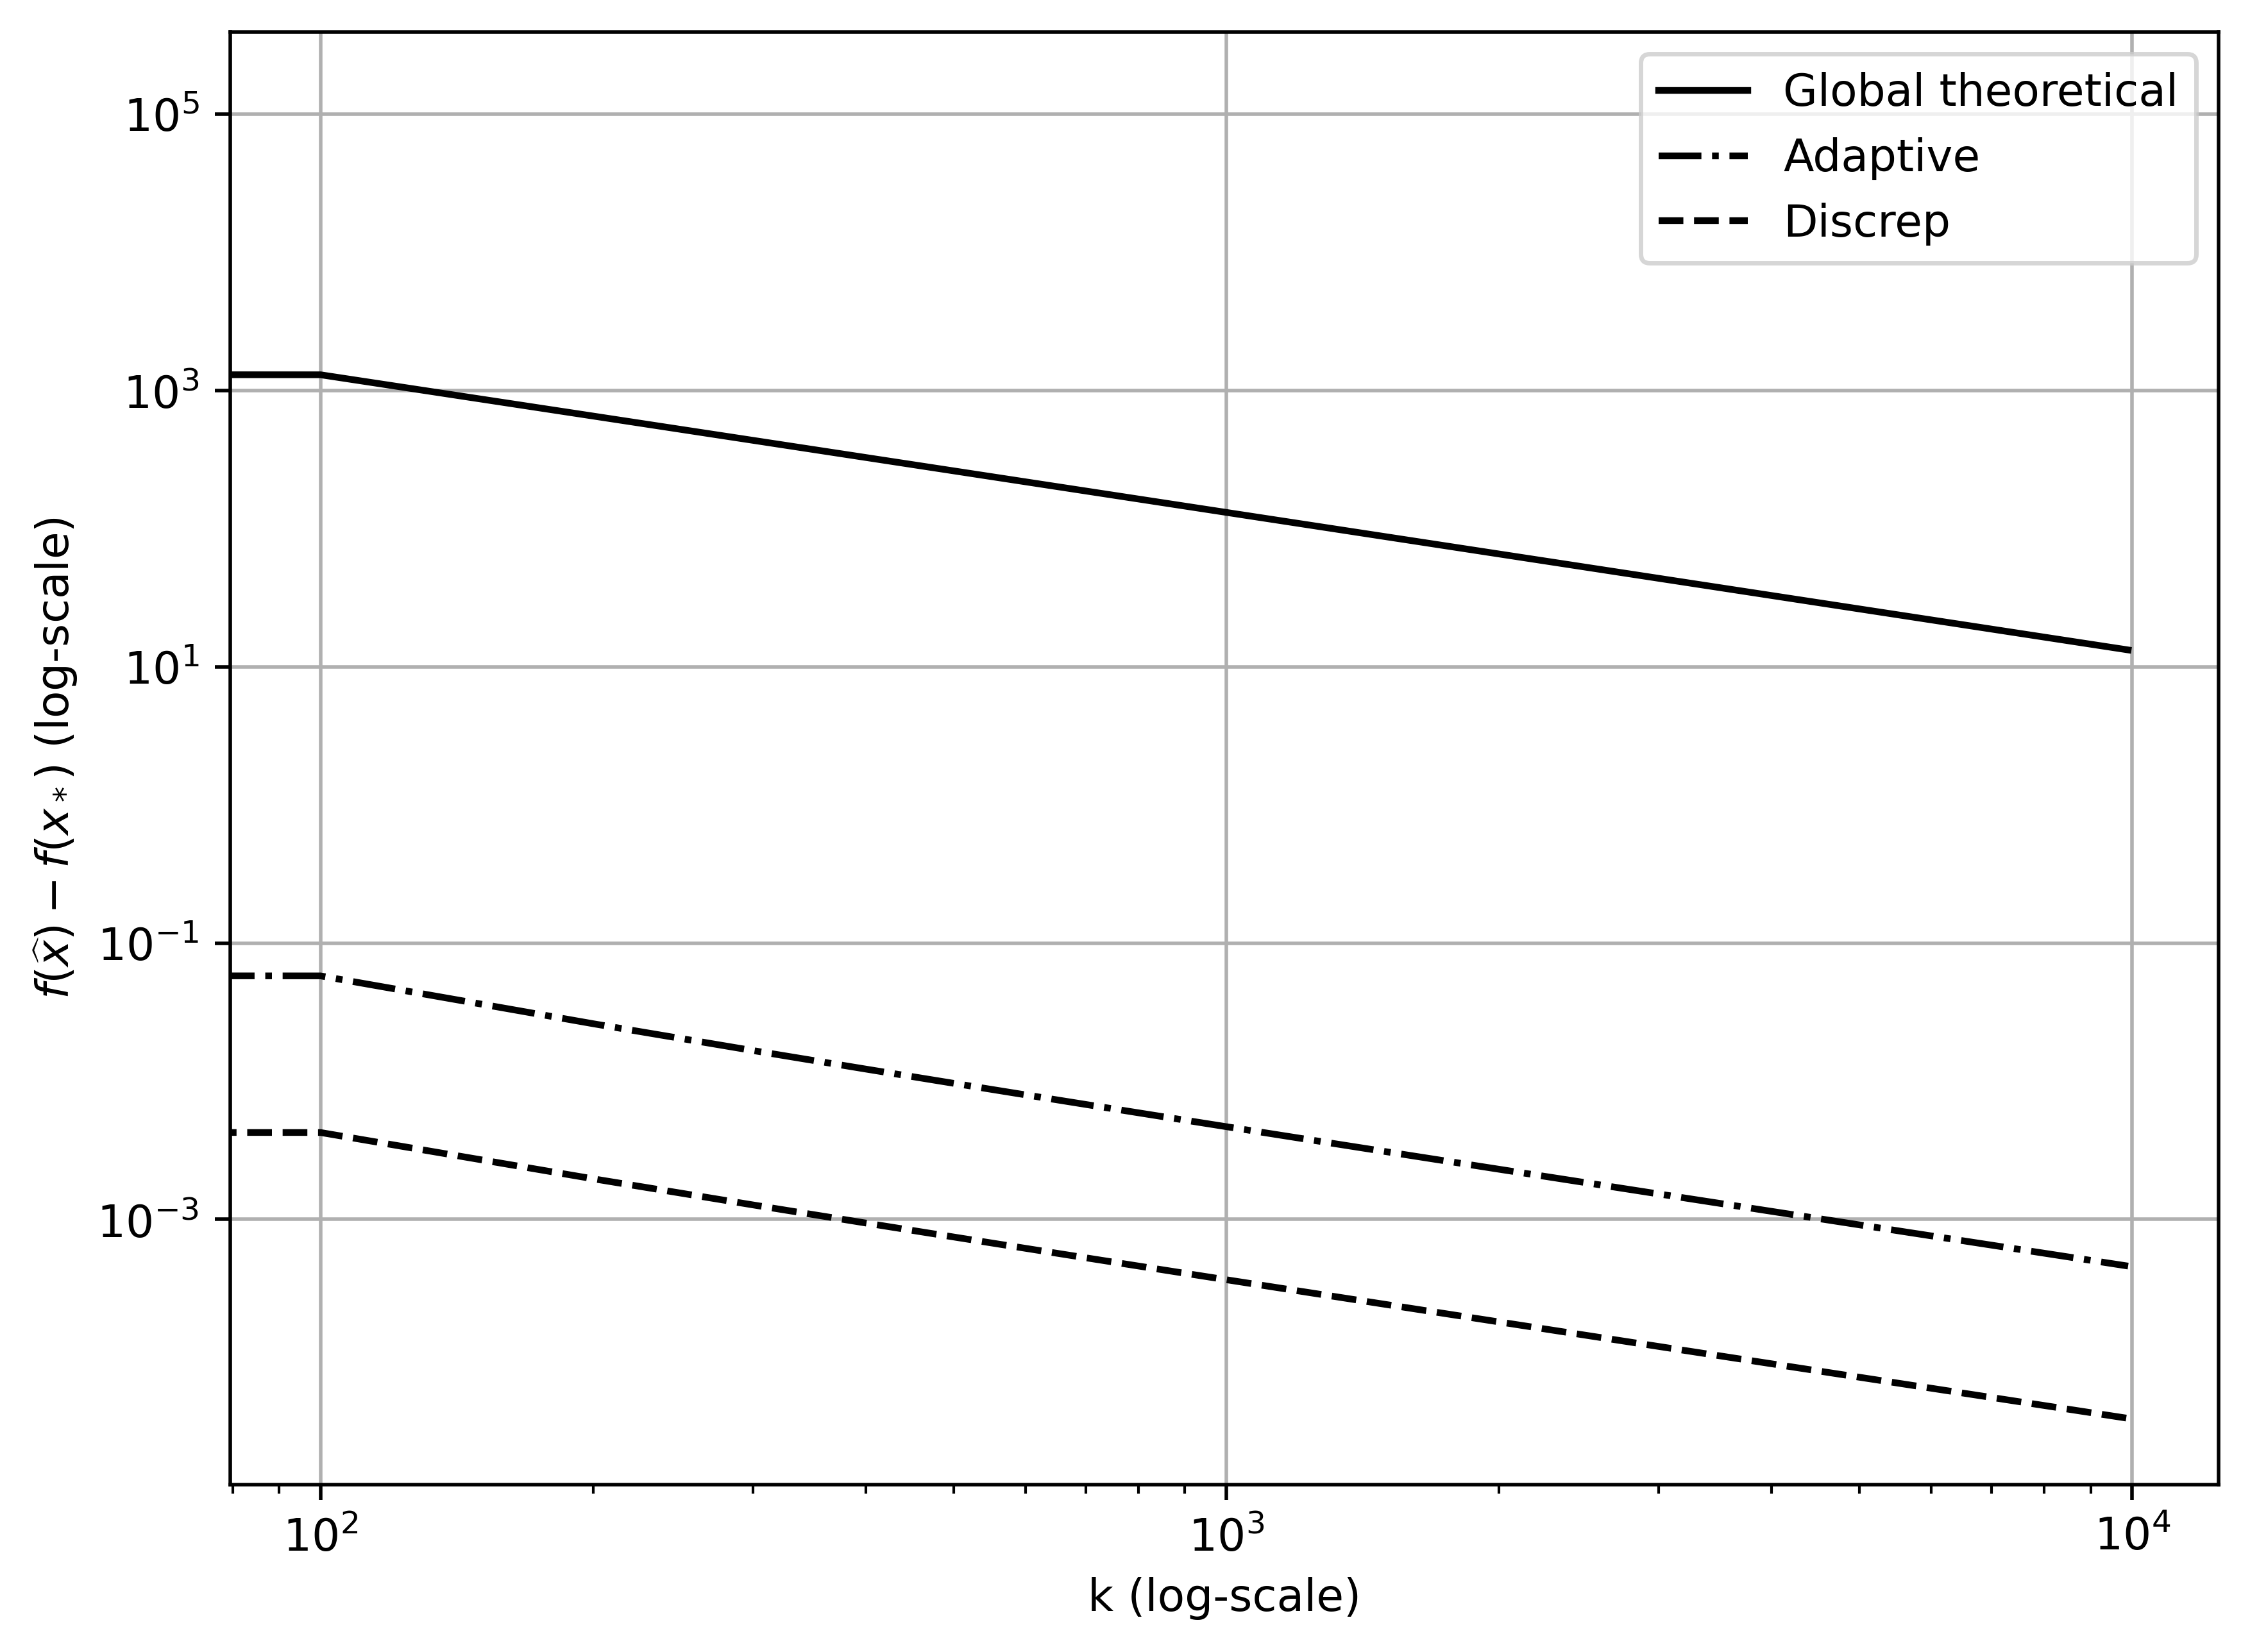
\includegraphics[width=\linewidth]{strong_convex_small_rad_f.png}
        \endminipage\hfill
        \label{res_strong_convex}
    \end{figure}
\end{frame}


\begin{frame} {[3 глава] Алгоритм рестартов при условии $\gamma$-роста.}
\begin{algorithm}[H]
    %\caption{Рестарты зеркального спуска при условии $\gamma$-роста.}
    \label{alg:rest_gamma}
    \KwData{$\varepsilon > 0$}
    \KwResult{$x_p$}
    $p \gets 0$\;
    $V(x_*, x_0) \gets V(x_*,x_0^0)$\;
    \While{$p > \log_2\left(\frac{V(x_*, x_0^0)}{\varepsilon}\right).$}{
        $x_{p}$ --- результат работы зеркального спуска и параметром $N_{p} = \frac{M^2 2^{\gamma}}{\mu_{\gamma}^2 2^{p(1 - \gamma)}} V(x_*, x_0^0)^{1 - \gamma}$\;
        $x_0 = \widehat{x_p}$\;
        $p=p+1$\;
    }
\end{algorithm}
\end{frame}


\begin{frame} {[3 глава] Эффективные оценки для алгоритма рестартов.}
\begin{block}{[Теорема]} \label{simple_restart}
    Пусть $f$ --- удовлетворяет условию $\gamma$-роста и также является $M$-липшицевой на $Q$ относительно некоторой функции Брегмана $V(x, y)$. В таком случае Алгоритм \ref{alg:rest_gamma} достигнет точности $\varepsilon$ после:
    \begin{equation}
    \begin{aligned}
       N = \mathcal{O} \left(\frac{2 M^2}{\mu_{\gamma}^2} \log_2{\frac{V(x_*, x_0^0)}{\varepsilon}} \right) \text{ при } \gamma = 1, \\
       N = \mathcal{O} \left( \frac{2 M^2}{\mu_{\gamma}^2 \varepsilon^{(\gamma-1)} } \left[1 - \frac{1} {V(x_*, x_0^0)^{(\gamma - 1)}}\right] \right) \text{ при } \gamma > 1,
    \end{aligned}
    \end{equation}
    причем будут справедливы неравенства:
    \begin{equation}
    \begin{aligned}
       V(x_*, \widehat{x_p}) \leq \varepsilon\\
       \text{ и }\\
       f(\widehat{x_p}) - f(x_*) \leq M \sqrt{2 \varepsilon}.
    \end{aligned}
    \end{equation}
\end{block}
\end{frame}

